\documentclass[a4paper, 11pt]{report}
\author{Valentin Clement}
\title{CLAW Fortran Compiler - Developer's Guide}

\usepackage[utf8]{inputenc}
\usepackage{verbatim}
\usepackage{moreverb}
\usepackage[english]{babel}
\usepackage[T1]{fontenc}
\usepackage{lmodern}
\usepackage{graphicx}
\usepackage{fancyhdr}
\usepackage{listings}
\usepackage{lastpage}
\usepackage[top=2cm, bottom=1cm, left=2cm, right=2cm]{geometry}
\usepackage{color}
\usepackage[table]{xcolor}
\usepackage{graphicx}
\usepackage{lipsum}
\usepackage{pgfplots}
\usepackage{CJKutf8}
\usepackage{glossaries}
\usepackage{xspace}

\setcounter{secnumdepth}{3}

\def\fortran{FORTRAN\xspace}
\def\clawfcomp{CLAW FORTRAN Compiler\xspace}
\def\omni{OMNI Compiler Infrastructure\xspace}
\def\xcodeml{XcodeML/F\xspace}
\def\ffront{\lstinline!F_Front!\xspace}
\def\fback{\lstinline!F_Back!\xspace}
\def\fpp{\lstinline!FPP!\xspace}
\def\clawfc{\lstinline!clawfc!\xspace}
\def\cx2x{\lstinline!CX2X!\xspace}

\makeglossaries

\newacronym{ast}{AST}{Abstract Syntax Tree}
\newacronym{ir}{IR}{Intermediate Representation}


%font change
\renewcommand{\familydefault}{\sfdefault}

\newcommand{\HRule}{\rule{\linewidth}{0.5mm}}
\newcommand{\nl}{\\[0.1cm]}
\newcommand{\s}{\vspace{0.3cm}}
%\newcommand{\emptypage}{\newpage \thispagestyle{empty} \mbox{}\newpage}
\newcommand{\emptypage}{}
\newcommand{\smore}{\vspace{0.6cm}}

\usepackage{caption}
\DeclareCaptionFont{white}{\color{white}}
\DeclareCaptionFormat{listing}{\colorbox{gray}{\parbox{\textwidth}{#1#2#3}}}
\captionsetup[lstlisting]{format=listing,labelfont=white,textfont=white}

\definecolor{darkgreen}{rgb}{0,0.4,0}
\definecolor{mauve}{rgb}{0.58,0,0.82}
\definecolor{Gray}{rgb}{0,0,0}
\definecolor{LightGray}{gray}{0.9}


\lstset{
    basicstyle=\footnotesize\ttfamily,
    keywordstyle=\color{orange}, %keywordstyle=\color{MidnightBlue}\bfseries,
    identifierstyle=\color{black},
    commentstyle=\color{darkgreen},
    stringstyle=\color{red},
    numbers=left,
    numberstyle=\color{Gray}\tiny,
    frame=bt, %frame=single,
    rulecolor=\color{Gray},
    numbersep=7pt,
    extendedchars=true,
    captionpos=b,
    breaklines=true,
    showspaces=false,
    showtabs=false,
    tabsize=2,
    xleftmargin=20pt,
    framexleftmargin=20pt,
    framexrightmargin=0pt,
    framextopmargin=0pt,
    framexbottommargin=0pt,
    showstringspaces=false,
    aboveskip=20pt,
    belowskip=20pt
}

\lstset{
	emph={parclass, sync, async, broadcast, scatter, gather, reduce, seq, conc, mutex},
	emphstyle={\color{orange}\bfseries}
}

\addto\captionsenglish{%
  \renewcommand{\listfigurename}{List of figures}%
	\renewcommand\refname{}
}

%Header and footer
\pagestyle{fancy}
\fancyhead{}
\fancyfoot{}

%Header definition
\renewcommand{\headrulewidth}{0.5pt}
\lhead{CLAW FORTRAN Compiler}
\rhead{Developer's Guide}

%Footer definition
\renewcommand{\footrulewidth}{0.5pt}
\lfoot{Version 0.1}
\rfoot{Page \thepage ~on \pageref{LastPage}}

\definecolor{grey}{rgb}{0.9,0.9,0.9} % Color of the box surrounding the title - these values can be changed to give the box a different color	

%remove indent for paragraph
\parindent0ex

\begin{document}

\thispagestyle{empty} % Remove page numbering on this page

%----------------------------------------------------------------------------------------
%	TITLE SECTION
%----------------------------------------------------------------------------------------
\colorbox{grey}{
	\parbox[t]{1.0\linewidth}{
		\centering \fontsize{35pt}{80pt}\selectfont % The first argument for fontsize is the font size of the text and the second is the line spacing - you may need to play with these for your particular title
		\vspace*{2cm} % Space between the start of the title and the top of the grey box
		
		\hfill \textbf{CLAW FORTRAN Compiler} \\
		\hfill Developer's Guide\par
		
		\vspace*{2cm} % Space between the end of the title and the bottom of the grey box
	}
}

\vfill

\begin{center}

\includegraphics[width=4cm]{resources/c2sm_logo.pdf} \\
\end{center}

\vfill % Space between the title box and author information

\begin{center}
Version 0.1, Last updated \today \\
Author: Valentin Clement
\end{center}
\HRule

\clearpage % Whitespace to the end of the page



\newgeometry{top=3cm,bottom=3cm,right=2cm,left=2cm}

%\emptypage
%\pagebreak
%\label{chapter:ack}
%\begin{center}
%\textsc{\LARGE Acknowledgment}
%\end{center}
%\input{acknowledgment}

%\emptypage
%\pagebreak
%\label{chapter:abstract}
%\begin{center}
%\textsc{\LARGE Abstract}
%\end{center}


\emptypage
\pagebreak
\tableofcontents



\chapter{Architecture}
\section{OMNI Compiler}
The \clawfcomp is based on the \omni. The \omni project provides a set of programs to build source-to-source translator for C or FORTRAN.

\subsection{The FORTRAN front-end}
The FORTRAN front-end is the program that parses FORTRAN source code and that generates the \gls{ir}. Its grammar is written in \lstinline|yacc| and the processing and \gls{ir} generation is written in \lstinline|C|.

%TODO gives a small example of the workflow inside the front-end.

\subsection{\xcodeml}
\xcodeml is the \gls{ir} used by the translator in the CLAW FORTRAN Compiler. This \gls{ir} is based on the XML format and is described in a specification document. It allows to have an high-level representation of FORTRAN 2008 programs.
%TODO add reference to specs.

Listing \ref{fortran1} is a simple FORTRAN program. Its \xcodeml \gls{ir} will be as shown in Listing \ref{xcodeml1}. A typical \xcodeml translation unit is composed of the followings sections: 
\begin{itemize}
\item Type table with all the type definitions used in the translation unit (Listing \ref{xcodeml1} line 6-24).
\item Global symbol table listing all the symbol at global scope (Listing \ref{xcodeml1} line 25-29).
\item Global declaration section listing the actual function or module declarations (Listing \ref{xcodeml1} line 30-82).
\end{itemize}

\lstinputlisting[label=fortran1, caption=Basic FORTRAN program, language=Fortran]{code/basic_fortran.f90}

\lstinputlisting[label=xcodeml1, caption=\xcodeml IR, language=xml]{code/basic_fortran.xml}

\subsection{The FORTRAN back-end}
The FORTRAN back-end is the program that decompiles \gls{ir} back to FORTRAN code. It is a simple Java program that implements a visitor patterns across the \gls{ast}.

\section{\clawfcomp}

The \clawfc is the program handed to the end-user. It performs all the needed step to have a source-to-source translation of a FORTRAN program. As shown in Figure \ref{fig:clawfc_main_workflow}, it is composed by various programs under-the-hood. The complete workflow is devided as follows: 

\begin{enumerate}
\item \textbf{FPP}: The FORTRAN source code is preprocessed by a standard FORTRAN preprocessor. Typically the one provided by the default compiler. 
\item \textbf{F\_Front}: The preprocessed FORTRAN source code is then parsed by the OMNI Compiler FORTRAN Front-end to produce the \xcodeml \gls{ir}.
\item \textbf{CX2X}: The \xcodeml is manipulated according to the rules of the CLAW directive language. The output is a valid \xcodeml \gls{ir}.
\item \textbf{F\_Back}: The \xcodeml \gls{ir} is decompiled to produce the transformed FORTRAN code. 
\end{enumerate}

\ffront{}, \fback{} are part of the \omni{}, \fpp{} is provided by the installed FORTRAN compiler. The \xcodeml to \xcodeml translator \cx2x{} is actively developed as part of the CLAW project.  

\begin{figure}[!ht]
  \centering
  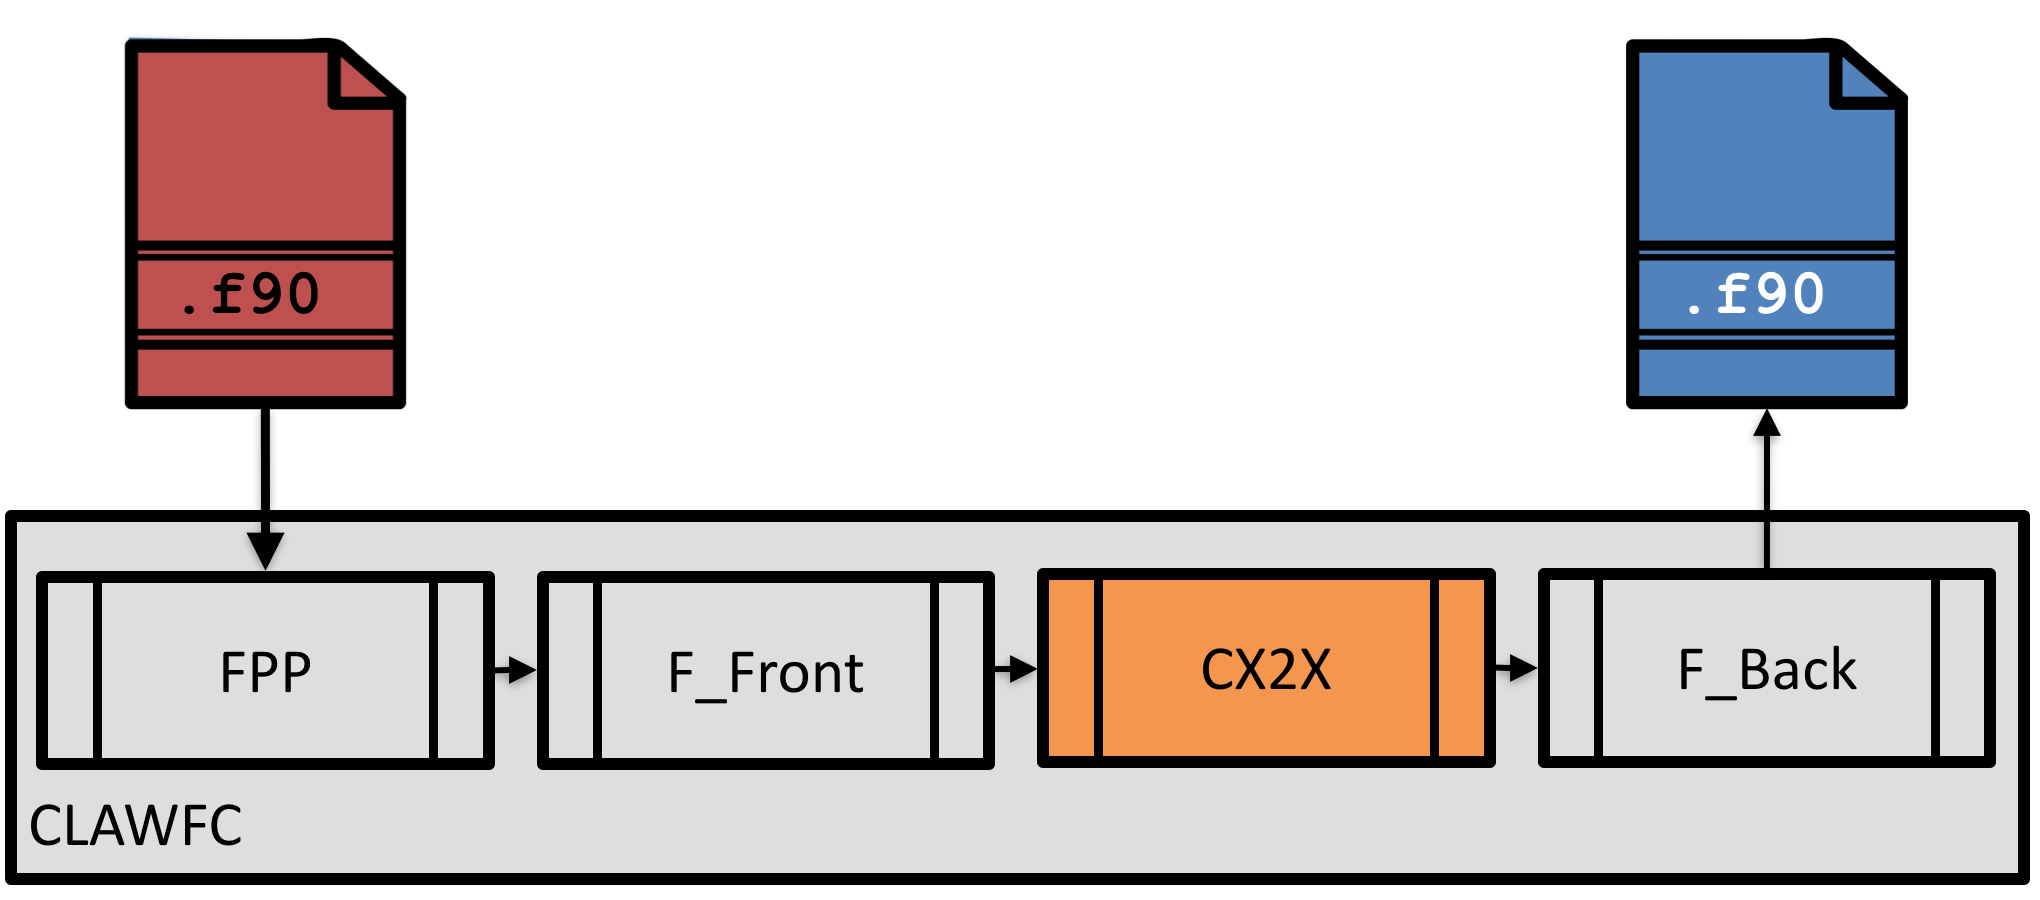
\includegraphics[width=0.8\textwidth]{resources/clawfc_global_workflow.png} \\
  \caption{CLAW FORTRAN Compiler main workflow.}
  \label{fig:clawfc_main_workflow}
\end{figure}

\section{CLAW \xcodeml to \xcodeml translator}
The \xcodeml to \xcodeml translator is the intelligence of the \clawfcomp. It understands the CLAW directive language and apply the corresponding transformation to the \xcodeml \gls{ast}.

\chapter{CLAW directive language}
%TODO add ref for the document
The CLAW directive language is specified in the "CLAW directive language specification". To validate and understand this language, a parser is needed in the heart of the \clawfcomp.

\section{CLAW directive language parser}
%TODO add ref to ANTLR
The CLAW directive language parser is based on the ANTLR project. ANTLR is a parser generator. From a grammar file, ANTLR generates a parser that is then used in the CLAW \xcodeml to \xcodeml translator to interpret the directives. 

\lstinputlisting[label=lst:antlr, language=Java, caption=ANTLR Grammar Example]{code/clawp.g4}

Listing \ref{lst:antlr} is a minimalist ANTLR example that support only two directives \lstinline|!$claw acc| or \lstinline|!$claw omp|.

In this grammar, there are two important sections, the parser and the lexer sections. The lexer section defined what will be recognized as a token. Here we defined the directives, the clauses but also more complex construct such as the \lstinline|IDENTIFIER| on line 28. It described the possible element to compose an identifier. This \lstinline|IDENTIFIER| can then be used later in the parser rules. 
The parser rules are defining the actual grammar of the language. In the case of this small example, the grammar says that the directive string must begins with \lstinline|claw| and then be followed by \lstinline|acc| or \lstinline|omp|. The code in \lstinline|{}| is java code that is triggered when the grammar rule is activated. In the example, it sets a value of the object returned after the analysis.
The \lstinline|@init{}| section allows to execute some Java code before triggering the actual parse. The \lstinline|@header{}| allows to insert Java code before the parser class.

\begin{lstlisting}[label=lst:antlr_cmd, caption=ANTLR parser generation command, language=bash]
javac -classpath <antlr_jar> org.antlr.v4.Tool -o . -package cx2x.translator.language.parser Claw.g4
\end{lstlisting}

The full CLAW ANTLR grammar is defined in the following file: \lstinline|omni-cx2x/src/cx2x/translator/language/parser/Claw.g4|

\chapter{Transformation}
A transformation class is the the basic representation of a manipulation of the \gls{ast} triggered by a directive. Each directive is implemented in its own transformation class. If the directive can be used as a block directive (with a \lstinline|!$end <directive>| directive), the class must inherits from the \lstinline!BlockTransformation!. Otherwise, it can inherits from the baisc \lstinline!Transformation! class.

\section{Type of transformation}
Transformations are divided into two distinct group. The independent and the dependent transformation. The first one, as its name implies, is performed independently of any other transformation. The dependent transformation, in the other hand, is applied only when it can be combined with another dependent transformation of the same kind in its group. Most of the transformations are independent. The best example for the dependent transformation is the loop fusion transformation. As shown in Listing \ref{lst:trans_dep}, there are two CLAW directive (line 4 and 9). These directives will trigger two dependent loop fusion transformations. The transformation engine will then analyze if the first one can be transformed with the second one. If so, the transformation will happen. Otherwise, the transformations are ignored.

\lstinputlisting[label=lst:trans_dep, caption=Loop fusion example, language=Fortran]{code/trans_dependent.f90}

\section{Transformation application order}

\section{Add a transformation}
A transformation in the \clawfc is represented as a class that inherits from the \lstinline|Transformation| base class or the \lstinline|BlockTransformation| class.

\chapter{\xcodeml and AST manipulation library}
As the \xcodeml \gls{ir} is based on the XML format, it can be manipulated with any language that can read and write XML files. It can even be manipulated by hand depending on the user's knowledge of the \xcodeml \gls{ir} specification. 
To ease this task, a small manipulation library is included in the \cx2x program. This library helps to traverse the \gls{ast}, add, modify or delete node.

\section{Traverse the \gls{ast}}

\section{Add nodes}

\section{Modify nodes}

\section{Delete nodes}

% GLOSSARY
\pagebreak
\glsaddall
\printglossaries

\emptypage
% FIGURES
\pagebreak
\listoffigures

%TABLES
\pagebreak
\listoftables

\emptypage
% LISTINGS
\pagebreak
\lstlistoflistings

% REFERENCES
%\input{references}

%\emptypage
%\input{appendix}

\end{document}
